\PassOptionsToPackage{unicode=true}{hyperref} % options for packages loaded elsewhere
\PassOptionsToPackage{hyphens}{url}
\documentclass[12pt,ignorenonframetext,aspectratio=169]{beamer}
\IfFileExists{pgfpages.sty}{\usepackage{pgfpages}}{}
\setbeamertemplate{caption}[numbered]
\setbeamertemplate{caption label separator}{: }
\setbeamercolor{caption name}{fg=normal text.fg}
\beamertemplatenavigationsymbolsempty
\usepackage{lmodern}
\usepackage{amssymb}
\usepackage{amsmath}
\usepackage{ifxetex,ifluatex}
\usepackage{fixltx2e} % provides \textsubscript
\ifnum 0\ifxetex 1\fi\ifluatex 1\fi=0 % if pdftex
  \usepackage[T1]{fontenc}
  \usepackage[utf8]{inputenc}
\else % if luatex or xelatex
  \ifxetex
    \usepackage{mathspec}
  \else
    \usepackage{fontspec}
\fi
\defaultfontfeatures{Ligatures=TeX,Scale=MatchLowercase}






%
\fi

  \usetheme[]{iqss}






% use upquote if available, for straight quotes in verbatim environments
\IfFileExists{upquote.sty}{\usepackage{upquote}}{}
% use microtype if available
\IfFileExists{microtype.sty}{%
  \usepackage{microtype}
  \UseMicrotypeSet[protrusion]{basicmath} % disable protrusion for tt fonts
}{}


\newif\ifbibliography


\hypersetup{
      pdftitle={Concept of cooperatives},
        pdfauthor={Deependra Dhakal},
          pdfborder={0 0 0},
    breaklinks=true}
%\urlstyle{same}  % Use monospace font for urls







% Prevent slide breaks in the middle of a paragraph:
\widowpenalties 1 10000
\raggedbottom

  \AtBeginPart{
    \let\insertpartnumber\relax
    \let\partname\relax
    \frame{\partpage}
  }
  \AtBeginSection{
    \ifbibliography
    \else
      \let\insertsectionnumber\relax
      \let\sectionname\relax
      \frame{\sectionpage}
    \fi
  }
  \AtBeginSubsection{
    \let\insertsubsectionnumber\relax
    \let\subsectionname\relax
    \frame{\subsectionpage}
  }



\setlength{\parindent}{0pt}
\setlength{\parskip}{6pt plus 2pt minus 1pt}
\setlength{\emergencystretch}{3em}  % prevent overfull lines
\providecommand{\tightlist}{%
  \setlength{\itemsep}{0pt}\setlength{\parskip}{0pt}}

  \setcounter{secnumdepth}{0}


  \usepackage{booktabs}
  \usepackage{longtable}
  \usepackage{emptypage}
  \usepackage{array}
  \usepackage{multirow}
  \usepackage{wrapfig}
  \usepackage{float}
  \usepackage{colortbl}
  \usepackage{pdflscape}
  \usepackage{tabu}
  \usepackage{threeparttable}
  \usepackage{threeparttablex}
  \usepackage[normalem]{ulem}
  \usepackage{rotating}
  \usepackage{makecell}
  \usepackage{xcolor}
  \usepackage{tikz} % required for image opacity change
  \usepackage[absolute,overlay]{textpos} % for text formatting
  \usepackage[utf8]{inputenc}
  \usetikzlibrary{mindmap,arrows,shapes,positioning,shadows,trees}
  \usepackage[skip=2pt]{caption}

  % this font option is amenable for beamer
  \setbeamerfont{caption}{size=\tiny}


%% IQSS overrides
\iqsssectiontitle{Outline}

\AtBeginSection[]{
  \title{\insertsectionhead}
  {
    \definecolor{white}{rgb}{0.776,0.357,0.157}
    \definecolor{iqss@orange}{rgb}{1,1,1}
    \ifnum \insertmainframenumber > \insertframenumber
    \frame{
      \frametitle{\iqsssectiontitleheader}
      \tableofcontents[currentsection]
    }
    \else
    \frame{
      \frametitle{Backup Slides}
      \tableofcontents[sectionstyle=shaded/shaded,subsectionstyle=shaded/shaded/shaded]
    }
    \fi
  }
}

\AtBeginSubsection[]{}

%%


  \title[]{Concept of cooperatives}



  \author[
        Deependra Dhakal
    ]{Deependra Dhakal}

  \institute[
    ]{
    GAASC, Baitadi \and Tribhuwan University
    }

\date[
      \today
  ]{
      \today
        }

\begin{document}

% Hide progress bar and footline on titlepage
  \begin{frame}[plain]
  \titlepage
  \end{frame}



\hypertarget{introduction}{%
\section{Introduction}\label{introduction}}

\begin{frame}{Definition}
\protect\hypertarget{definition}{}
\begin{itemize}
\tightlist
\item
  A cooperative is an autonomous association of people who voluntarily
  cooperate for their mutual social, economic, and cultural benefit.
\item
  Includes non-profit community organizations and businesses that are
  owned and managed by the people who use its services (a consumer
  cooperative) or by the people who work there (a worker cooperative) or
  by the people who live there (a housing cooperative).
\item
  In short: ``a jointly owned enterprise engaging in the production or
  distribution of goods or the supplying of services, operated by its
  members for their mutual benefit, typically organized by consumers or
  farmers.''
\item
  Co-operatives frequently have social goals which they aim to
  accomplish by investing a proportion of trading profits back into
  their communities.
\item
  The Rochdale Society of Equitable Pioneers, founded in 1844, is
  usually considered the first successful cooperative enterprise. They
  set up the society to open their own store selling food items they
  could not otherwise afford.
\end{itemize}
\end{frame}

\begin{frame}{Principles\footnote<.->{Adopted by the international
  cooperative alliance in 1995}}
\protect\hypertarget{principles}{}
\footnotesize

\begin{enumerate}
\tightlist
\item
  Voluntary and open membership
\end{enumerate}

\begin{itemize}
\tightlist
\item
  Cooperatives are open to all people willing to volunteer to use its
  services and willing to accept the responsibilities of membership,
  without gender, social, racial, political or religious discrimination.
\end{itemize}

\begin{enumerate}
\setcounter{enumi}{1}
\tightlist
\item
  Democratic member control
\end{enumerate}

\begin{itemize}
\tightlist
\item
  Those who buy the goods or use the services of the cooperatives also
  actively participate in setting policies and making decisions.
\end{itemize}

\begin{enumerate}
\setcounter{enumi}{2}
\tightlist
\item
  Members' economic participation
\end{enumerate}

\begin{itemize}
\tightlist
\item
  Members contribute equally to and democratically control the capital
  of the cooperative.
\item
  Benefits are distributed proportionally to each member's level of
  participation in the cooperative, for instance, by a dividend on sales
  or purchases, rather than according to capital invested.
\end{itemize}
\end{frame}

\begin{frame}{}
\protect\hypertarget{section}{}
\begin{enumerate}
\setcounter{enumi}{3}
\tightlist
\item
  Autonomy and independence
\item
  Education, training and information
\item
  Cooperation among cooperatives
\item
  Concern for community
\end{enumerate}
\end{frame}

\hypertarget{organizationstructures}{%
\section{Organization/structures}\label{organizationstructures}}

\begin{frame}{}
\protect\hypertarget{section-1}{}
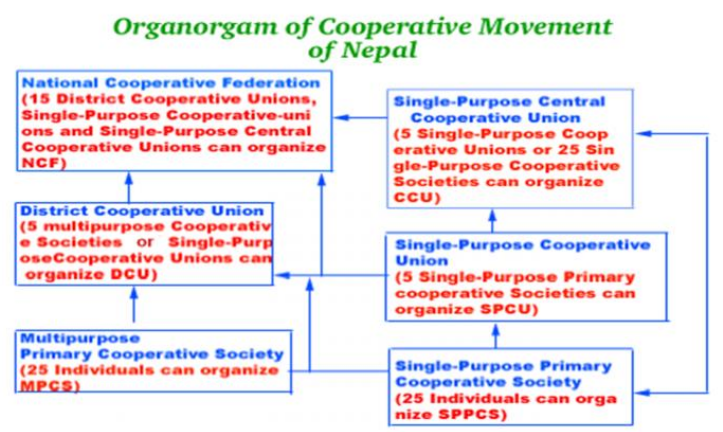
\includegraphics[width=0.8\linewidth]{./figs/organogram_cooperative_movement}
\end{frame}

\begin{frame}{}
\protect\hypertarget{section-2}{}
\footnotesize

\begin{enumerate}
\item
  Producer co-operatives: Some co-operatives process and market their
  members' products and services directly while others may also sell the
  input necessary to their members' economic activities. Examples:
  Agriculture cooperatives, pooling of equipment, advisory services,
  etc.
\item
  Multi-stakeholder co-operatives: The membership of these co-operatives
  is made of different categories of members who share a common interest
  in the organization. Examples: home care services, health services,
  community services, etc.
\item
  Worker co-operatives: The purpose of these co-operatives is to provide
  their members with work by operating an enterprise. The co-operatives
  are owned by their employee members. Examples: forestry, leisure,
  production and manufacturing, tourism, communications and marketing,
  etc.
\end{enumerate}
\end{frame}

\begin{frame}{}
\protect\hypertarget{section-3}{}
\begin{enumerate}
\setcounter{enumi}{3}
\item
  Worker-Shareholder co-operatives: These are incorporated co-operatives
  that hold partial ownership of the business in which the co-operative
  members are employed. Because of its share capital, the co-operative
  may participate in the management of the business and the workers may
  influence work organization. Examples: production and manufacturing,
  technology, etc.
\item
  Consumer co-operatives: A consumers' cooperative is a business owned
  by its customers. Employees can also generally become members. Members
  vote on major decisions and elect the board of directors from among
  their own number. They provide their members with goods and services
  for their personal use. Examples: Food, credit unions, housing,
  insurance co-operatives, etc.
\end{enumerate}
\end{frame}

\hypertarget{roles-of-cooperative-in-commercial-farming}{%
\section{Roles of cooperative in commercial
farming}\label{roles-of-cooperative-in-commercial-farming}}

\begin{frame}{}
\protect\hypertarget{section-4}{}
\footnotesize

\begin{itemize}
\tightlist
\item
  Agricultural cooperatives play an important role in food production
  and distribution, and in supporting long-term food security.
\item
  Agricultural cooperatives play an important role in supporting small
  agricultural producers and marginalized groups such as young people
  and women.
\item
  Cooperatives offer small agricultural producers opportunities and a
  wide range of services, including improved access to,

  \begin{itemize}
  \tightlist
  \item
    markets,
  \item
    natural resources,
  \item
    information,
  \item
    communications,
  \item
    technologies,
  \item
    credit,
  \item
    training, and
  \item
    warehouses.
  \end{itemize}
\end{itemize}
\end{frame}

\begin{frame}{}
\protect\hypertarget{section-5}{}
\footnotesize

\begin{itemize}
\tightlist
\item
  Facilitate smallholder producers' participation in decision-making at
  all levels, support them in securing land-use rights, and negotiate
  better terms for engagement in contract farming and lower prices for
  agricultural inputs such as seeds, fertilizer and equipment.
\item
  Through this support, smallholder producers can secure their
  livelihoods and play a greater role in meeting the growing demand for
  food on local, national and international markets, thus contributing
  to poverty alleviation, food security and the eradication of hunger.
\item
  Agricultural cooperatives also promote the participation of women in
  economic production

  \begin{itemize}
  \tightlist
  \item
    women are able to unite in solidarity and provide a network of
    mutual support to overcome cultural restrictions to pursuing
    commercial economic activities.
  \item
    For example, women-only cooperatives in South Asia facilitate
    economic independence and improve the social standing of women
    through their active participation in businesses and management.
  \end{itemize}
\end{itemize}
\end{frame}

\hypertarget{cooperatives-laws-and-by-laws}{%
\section{Cooperatives laws and
by-laws}\label{cooperatives-laws-and-by-laws}}

\begin{frame}{National cooperative federation of Nepal (NCFN)}
\protect\hypertarget{national-cooperative-federation-of-nepal-ncfn}{}
\begin{itemize}
\tightlist
\item
  Established in June 20, 1993 under the Co-operative Act, 1992
\item
  The apex body of the cooperative movement of all types and levels of
  cooperatives organized on the basis of universally accepted
  cooperative values and principles.
\item
  Represents in government, national and international forum on behalf
  of all cooperatives.
\item
  There are more than 24 thousand Primary Cooperatives, 223 District
  Level Cooperative Unions, 14 Central Cooperative Unions and 1 National
  Cooperative Bank under the umbrella of NCFN.
\item
  There are more than 3.2 million cooperative members including around
  42 percent women membership. (Source: Department of Cooperatives, July
  15, 2011)
\item
  NCFN is a member of International Cooperative Alliance (ICA), Geneva.
  It is also affiliated with the Network for the Development of
  Agricultural Cooperatives (NEDAC), Thailand.
\end{itemize}
\end{frame}




\end{document}
